% To create a slide, use the following:
% \begin{frame}{TITLE}
%     BODY
% \end{frame}

% To create a slide with a bullet list, use the following:
% \begin{frame}{TITLE}
%     \begin{itemize}
%         \item ITEM 1
%         \item ITEM 2
%     \end{itemize}    
% \end{frame}

% To create a slide with numbered list, use the following:
% \begin{frame}{TITLE}
%     \begin{enumerate}
%         \item ITEM 1
%         \item ITEM 2
%     \end{enumerate}
% \end{frame}

% To create a slide with a graphic:
% 1. Add the graphic to this folder (named picture.png)
% 2. Use the following:
% \begin{frame}{TITLE}
%     \centering
%     \includegraphics[height=0.7\textheight,width=0.7\textwidth,keepaspectratio]{picture.png}
% \end{frame}

% To create a slide with two columns, use the following:
% \begin{frame}{TITLE}
%     \begin{columns}
%         \begin{column}{0.5\textwidth}
%             COLUMN 1 BODY
%         \end{column}
%         \begin{column}{0.5\textwidth}
%             COLUMN 2 BODY
%         \end{column}
%     \end{columns}
% \end{frame}
\begin{frame}{WebSocket Progress}
    Frontend WebSockets integrated with callbacks
    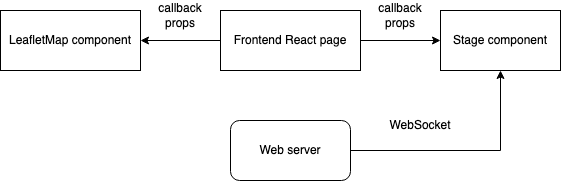
\includegraphics[height=0.7\textheight,width=0.7\textwidth,keepaspectratio]{mm_1-24_callbacks.png}
\end{frame}

\begin{frame}{GeoJSON Rendering}
    Add/remove GeoJSON layers from map
\end{frame}

\begin{frame}{Image Chunking and S3 Buckets}
    \begin{enumerate}
        \item Image chunking
        \item S3 Bucket Request
    \end{enumerate}
\end{frame}

\begin{frame}{Fixed Dockerfiles using Poetry}
    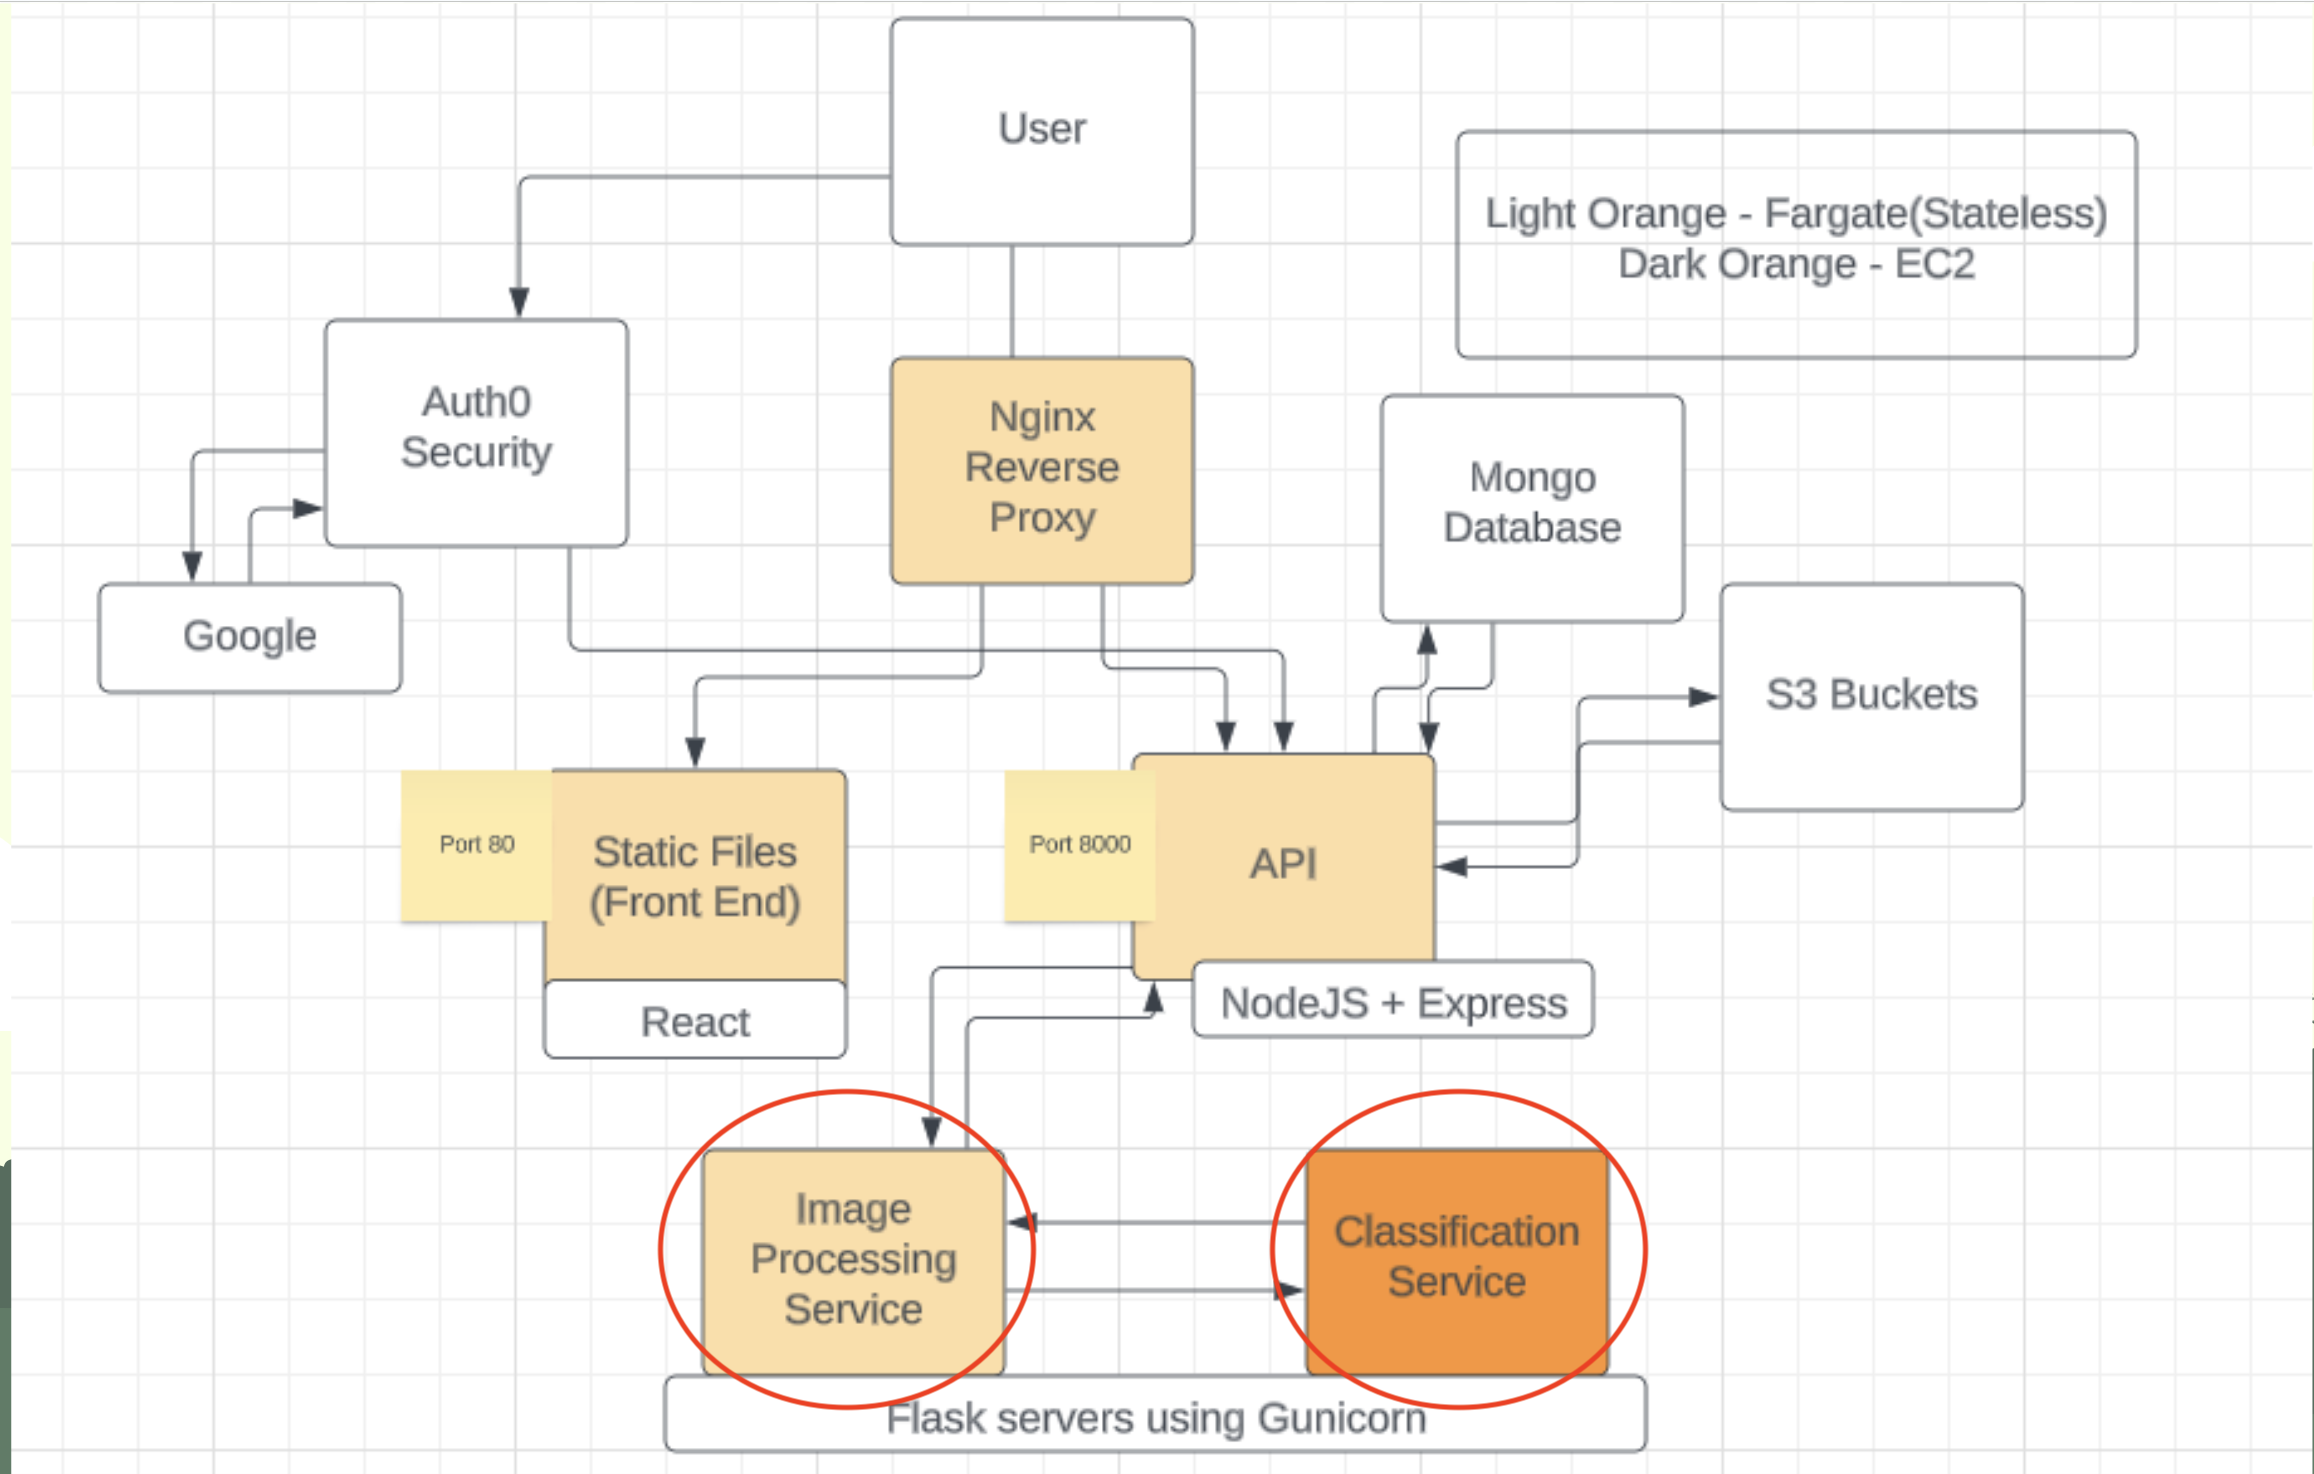
\includegraphics[height=0.7\textheight,width=0.7\textwidth,keepaspectratio]{mm-images/Screenshot 2024-01-24 at 1.33.57 PM.png}
    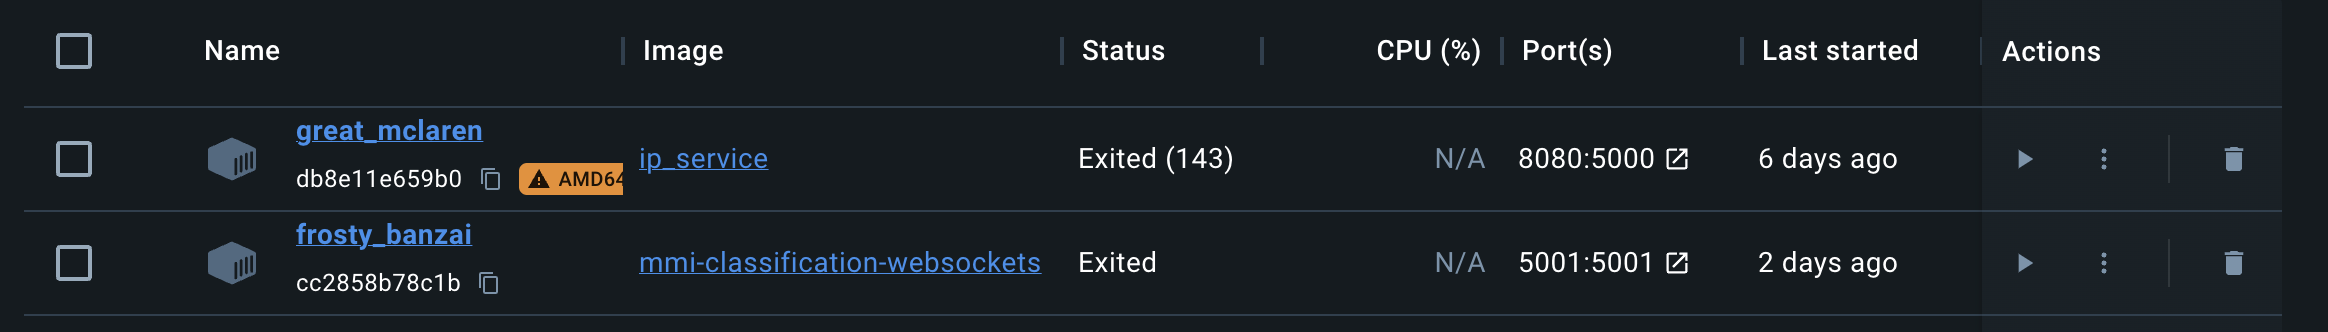
\includegraphics[height=0.7\textheight,width=0.7\textwidth,keepaspectratio]{mm-images/Screenshot 2024-01-24 at 1.35.48 PM.png}
\end{frame}

\begin{frame}{Misc. Frontend}
    \begin{enumerate}
        \item Map fullscreen
        \item Multiple GeoJSON toggle
    \end{enumerate}
    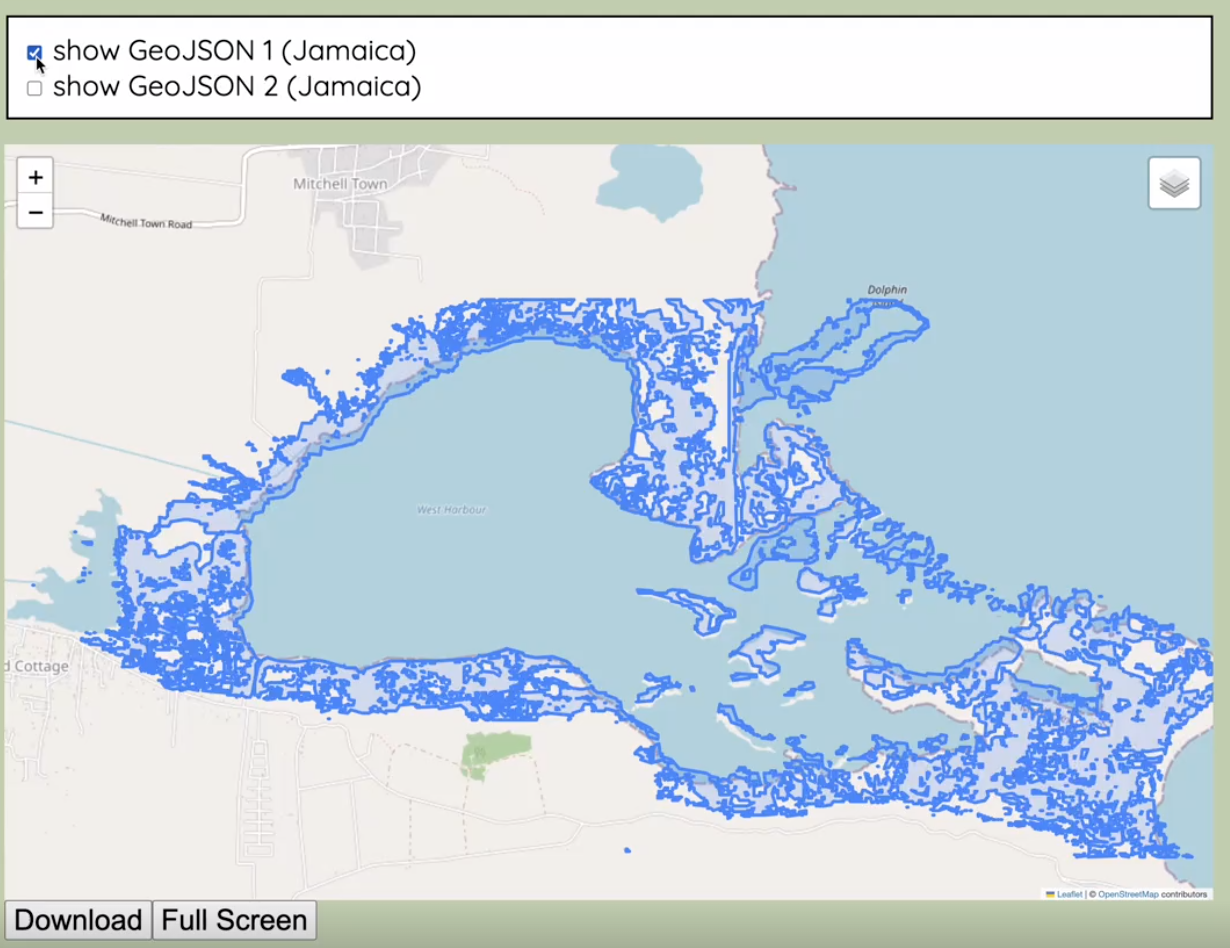
\includegraphics[height=0.7\textheight,width=0.7\textwidth,keepaspectratio]{mm_1-24_fullscreen.png}
\end{frame}

\begin{frame}{No Drone Imagery Accuracy}
    \centering
    98.13\% Accuracy, 98.22\% with Drone
    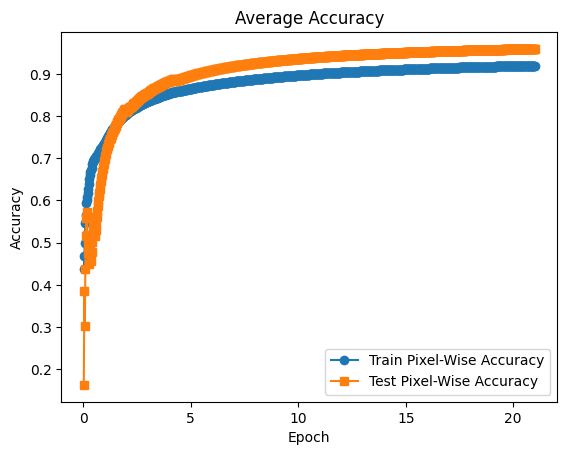
\includegraphics[height=0.7\textheight,width=0.7\textwidth,keepaspectratio]{mm-images/AvgAcc.png}
    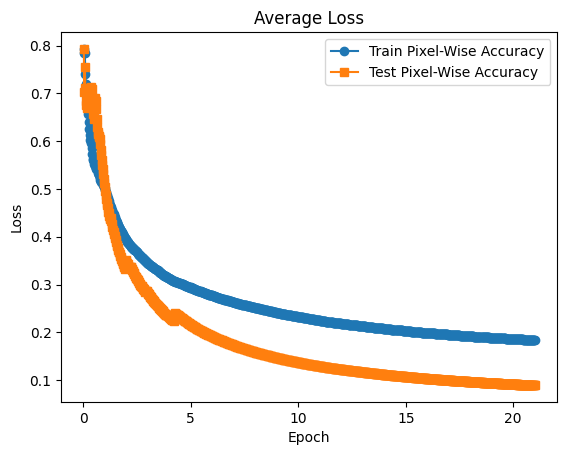
\includegraphics[height=0.7\textheight,width=0.7\textwidth,keepaspectratio]{mm-images/AvgLoss.png}
\end{frame}

\begin{frame}{Trouble Predicting Satellite Imagery}
    \centering
    Model Not 0-1
    ModelOutput
    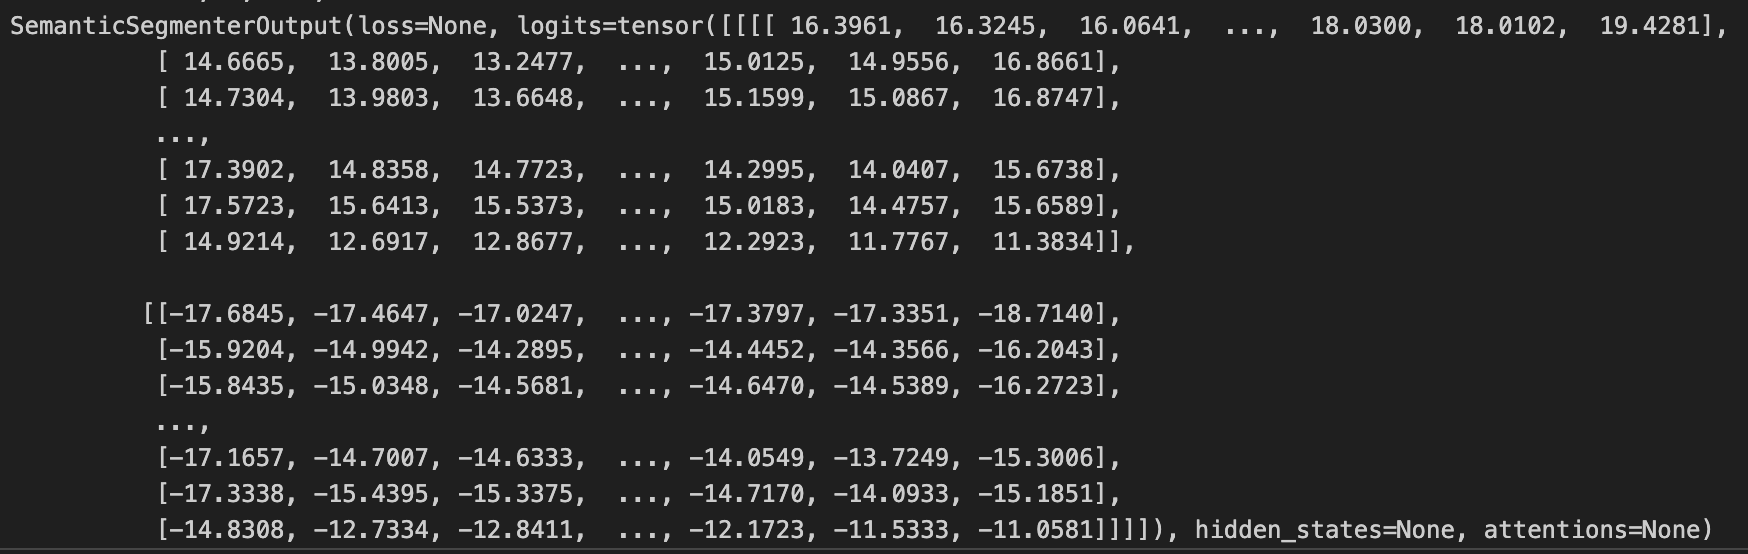
\includegraphics[height=0.7\textheight,width=0.7\textwidth,keepaspectratio]{mm-images/ModelOutput.png.png}
    Logits
    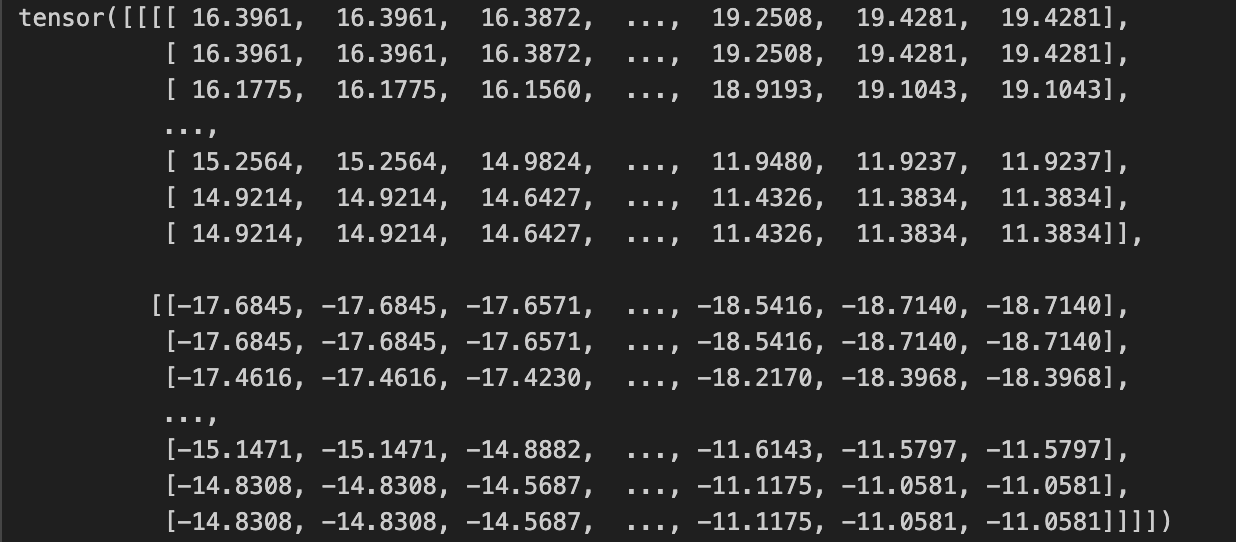
\includegraphics[height=0.7\textheight,width=0.7\textwidth,keepaspectratio]{mm-images/Logits.png.png}
\end{frame}